\section{Service Mesh}
\label{sec:background:service-mesh}

In the previous sections we discussed the evolution in deployment models (\cref{sec:background:containers}) and how this caused a shift in system design, based on decoupling business logic into logical services (\cref{sec:background:soa}). We then went on to briefly introduce \gls{k8s} and several related concepts (\cref{sec:background:soa}). In this section, we build on top of the topics discussed in the background chapter and introduce the \gls{sm} architecture which is at the core of the work presented in this thesis. A style of architecture that builds on top of the \gls{k8s} ecosystem which aims to solve the communicative challenges caused by service-oriented design.

% This section introduces a service mesh to the user
% What is a service mesh
% What does a service mesh try to solve
% Why is it becoming a thing now
% Is it a overhyped technology


\begin{figure}[!t]
    \centering
    
    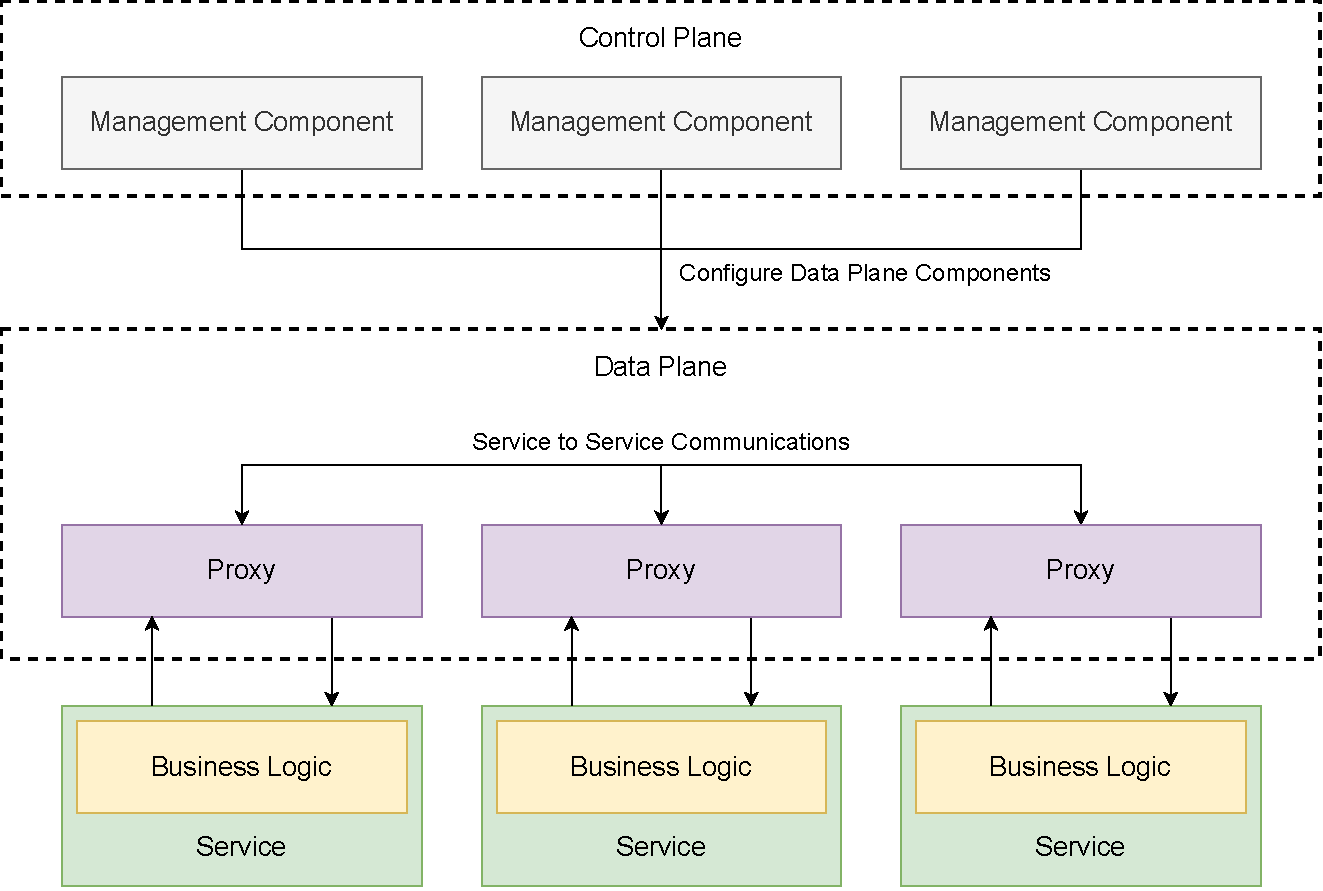
\includegraphics[width=\linewidth]{2_background/figures/service-mesh-architecture.pdf}

    \caption[Service Mesh Architecture]{\Gls{sm} architecture}
    \label{fig:service-mesh-architecture}
\end{figure}

% Context
% Short intro service mesh, how it can add to latency/overhead
A \gls{sm} is a dedicated layer of networking infrastructure that sits between logical software services and aims to solve some communicative challenges introduces by a \gls{soa}. The terminology was introduced in the last decade \cite{service-mesh-hype}, and several systems adhering to this architecture have seen the light of day since. The premise of introducing additional observability in the system, increasing the reliability of it while also adding security best practices to little or no additional lines of application code made this technology a hot topic in the field. However, this technology does not come in the form of a zero cost offering. The \gls{sm} architecture introduces additional machinery to achieve its goals and is depicted in \cref{fig:service-mesh-architecture}. The components that make up a \gls{sm} can be divided into two  categories. A set of management components that constitute the \textit{Control Plane} and a set of components that handle the network traffic referred to as the \textit{Data Plane}.

\subsection{Data Plane}
\label{sec:background:service-mesh:data-plane}

The data plane is what actually defines the dedicated layer of networking infrastructure, it is what creates the mesh. It is created by placing \textit{proxies} in front of the logical services. The goal of these proxies is to intercept all traffic to and from a given service. All service-to-service communications, and direct requests to a service go through these proxies. Notably, these proxies are \textit{Layer 7-aware TCP proxies} like many popular general purpose proxies such as \textit{HAProxy} or \textit{NGINX}. Although the choice of proxy is an implementation detail, most \gls{sm} use a proxy that has a focus on high performance and a feature set that aligns with the many benefits a \gls{sm} can give (as discussed in \cref{sec:background:service-mesh:benefits}).

By introducing these proxies into the system, an increase in system resources is to be expected. More importantly, the introduction of a network proxy leads to an increase in the amount of network hops in the data path for each packet. The downside of this is that this therefore leads to an increase in request latency and can cause for scalability concerns. In this thesis, we take an experimental approach to quantify the performance overheads caused by a \gls{sm} system. Therefore, we will focus on the impact of the data plane components.


\subsection{Control Plane}
\label{sec:background:service-mesh:control-plane}

A second set of components makes up the control plane of a \gls{sm} system. This set of components is used to manage and facilitate the functionalities of a \gls{sm}. It provides coordination and configuration for the data plane proxies and performs functions such as service discovery and metric aggregation. Another component often found in the control plane of \gls{sm} is a \textit{Certificate Authority}, which issues TLS certificates to the data plane proxies enabling them to encrypt data. 

Compared to the data plane components, the control plane components have a lesser impact on the performance of systems. First, it does not affect the network traffic in the data path directly, and only has an impact on system resources. Furthermore, this impact is mostly static, as there often is just one instance of each component which provides a sharp contrast to the most common data plane design which results in a proxy per individual service. 

\subsection{Benefits of a Service Mesh}
\label{sec:background:service-mesh:benefits}

To understand the benefits of a \gls{sm} system, we first need to understand which challenges such a system is trying to solve. As previously discussed in \cref{sec:background:soa}, we expanded on the benefits of a service-oriented approach, but also briefly explained some downsides of such an architecture. In short, it adds another layer of complexity into a system that comes in the form of communicative overhead. Services have to deal with the inherent by-products of communications and networking. Network connections can fail, services can crash or experience downtime, services now have to deal with load balancing and service discovery just to name a few of those challenges. 

The \gls{sm} architecture and the systems that implement this try to address these challenges in a uniform fashion. It provides a way to implement distributed systems best practices without having to modify the business logic that makes up a logical service. The advantages of a \gls{sm} architecture can be categorized into four groups.

\begin{enumerate}[leftmargin=3\parindent]
    \item \textbf{Observability}
    The first set of features and advantages related to a \gls{sm} system deals with the observability of communications. The data plane of a service mesh can log the details of network request in a uniform manner. Furthermore, it captures metrics such as request latencies, request payload sizes, request volumes and status codes to name a few. Another desirable aspect is that it allows operators to view and create service topology maps, depicting the relations between services or inspect and trace individual requests throughout a system.
    
    \item \textbf{Reliability}
    Every engineer and user wants a reliable system; however, there are many challenges that one has to solve to make a system reliable. Network connections can fail, services can crash or experience downtime or a new software update can cause compatibility issues. A \gls{sm} tries to solve some of these problems by introducing a set of reliability features. Some of these include the ability to automate and configure request retries and timeouts. Another feature that helps in this area is the ability to perform traffic splitting and shifting, often used for \textit{canary deployment}\footnote{A  canary deployment is a software rollout strategy that is based on staged releases. The core idea is that the software is only available to a particular subset of users, which is slowly incremented over time. This practice serves as an early warning and can minimize the impact of failed deployments.}.

    \item \textbf{Security}
    A major advantage of using a \gls{sm} system is related to the security related features that it provides. One of the major challenges of modern IT systems is related to security and data privacy. How can we make sure that data cannot be observed by bad actors and limit or control the access within a system? Due to the design of the data plane all communications go through a network proxy (see \cref{sec:background:service-mesh:data-plan}). This enables a service mesh to automatically encrypt all data transfers in service-to-service communications through modern encryption standards. Furthermore, it enables the operator to configure access control for said services with finer granularity.
    
    \item \textbf{Programmability}
    A final category of features that a \gls{sm} provides is related to the programmability of such systems. The first set of programmability features is related to the type of proxy used in the data plane. Due to the layer 7 aware network proxies that it uses, it can make decisions based on application level protocol details. This allows an operator to configure networking, routing and load balancing on application level details such as \textit{HTTP} headers, paths or \textit{Kafka} topics. The second set of features that enable an additional layer of programmability is due to the extensibility features often found within the proxies used in \gls{sm} systems. Many of the popular data plane proxies such as \textit{Envoy} allow the user to extend the default feature set\footnote{\url{https://www.envoyproxy.io/docs/envoy/latest/extending/extending}}.

\end{enumerate}


\subsection{Alternatives to the Service Mesh Architecture}
\label{sec:background:service-mesh:alternatives}

We discussed the set of challenges that a \gls{sm} tries to solve, however, this set of challenges related to communications have existed long before the notion of a \gls{sm} even existed. How did we solve these challenges before, and what are some alternative solutions? 

One approach would be to manually configure and handle all the aspects and features that a \gls{sm} architecture implements. This would be the best performing option, requires no additional machinery to implement and allows the software engineers to use any language or framework, that best suit their needs to implement various logical services. The downside of this approach is that it will most likely lack in uniformity, and requires a significant effort from the software engineers to implement in a microservices architecture, as it would mean that engineers would have to manually manage and implement the intricacies of networking best practices.

Another approach used was to utilize another design pattern that implements an \gls{esb}, an open standard, message-based, distributed integration infrastructure that provides routing, invocation and mediation services to facilitate the interactions of disparate distributed applications and services in a secure and reliable manner \cite{menge2007enterprise}. This dedicated piece of infrastructure combines  Message-Oriented Middleware (MOM), web services, transformation and routing intelligence as a backbone for Service-Oriented Architecture.  The most significant difference with the service mesh architecture, is that the services within such an \gls{esb} architecture relied on the infrastructure and middlewares of it. In a \gls{sm} architecture, the services are not aware of any topology changes or that their networking traffic is being intercepted at all. This is a key difference and important to note, as it provides a clear separation of concerns from the \gls{esb} architecture frequently used in the 90s.

\begin{figure}[!t]
    \centering
    
    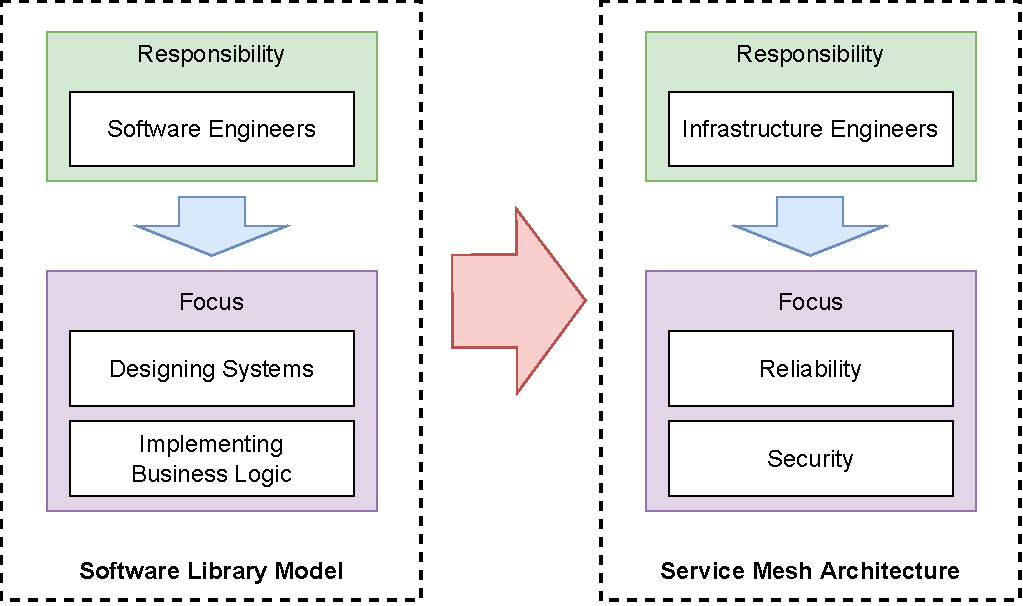
\includegraphics[width=0.8\linewidth]{2_background/figures/responsibility-model.pdf}

    \caption[Service Mesh Responsibility Model]{\Gls{sm} responsibility model. Compares the shift in responsibilities compares to the software library approach and shows that it can provide a clear separation of concerns for the stakeholders involved. It allows the stakeholders involved to focus and work on the objectives that align with their roles.}
    \label{fig:service-mesh-responsibility-model}
\end{figure}

Another common alternative was already briefly touched upon in  \cref{sec:background:soa:challenges}, in which we introduced the software library-based approach that did not rely on additional machinery to be implemented. The software libraries are used to implement a uniform client and server interface. With a focus on load balancing mechanisms, fault tolerance with retry and timeout feature sets the software library implements many of the features and mechanisms present in a \gls{sm} system. This approach can be the most performant option, as it does not introduce additional network hops and complex systems. However, a clear downside of such an approach is that this would mean that software engineers would be limited to use a single programming language to implement all business logic, or maintain multiple software libraries to support different technology stacks. Furthermore, an update to such a library would mean that all the services running that library would require an update as well. 

In \cref{fig:service-mesh-responsibility-model} we compare the most common alternative to the \gls{sm} architecture and shows the shift in responsibility that it caused. By using a \gls{sm} architecture, the infrastructure engineers maintain the \gls{sm} system. The features that a \gls{sm} provides align with the goals and objectives that such a stakeholder has, such as maintaining a reliable platform and having a security first mindset. For software engineers this meant that they do not have to maintain, update and implement these libraries and can focus on system design and implementing business logic instead. This provides a clear separation of concerns and allows the stakeholders to focus more on the goals and objectives aligned with their respective roles.